\section{Aplicações Cliente}\label{sec32}

Disponibilizam-se aplicações cliente em dispositivos móveis \textit{Android} (\textit{smartphones} e \textit{tablets}) e dispositivos \textit{desktop}, através do \textit{browser}. Na implementação das mesmas teve-se em atenção conceitos como \textit{responsive}, pois tal permite, não só, uma melhor experiência de utilizador, como também, uma interface mais apelativa aos diversos dispositivos suportados.

Realizou-se uma pesquisa pelas aplicações já existentes de maneira a estar cientes do que se pode encontrar no mercado e comparar com o que o sistema Smart Stock oferece, como se pode observar na tabela \ref{tab-comparacao-duas-aplicacoes}. 

\begin{table}
	\centering
	\caption{Comparação do sistema Smart Stocks com outros}\vspace{2mm}
	\label{tab-comparacao-duas-aplicacoes}
	\resizebox{\textwidth}{!}{%
		\begin{tabular}{m{6cm}|C{3cm}|C{3cm}|C{2cm}}
			\textbf{} & \textbf{Smart Stocks} & \textbf{OutOfMilk} & \textbf{Bring!}\\
			\hline Aplicação Móvel & \cmark & \cmark & \cmark \\
			\hline Aplicação Web & \cmark & \cmark & \cmark \\
			\hline Listas de Compras & \cmark & \cmark & \cmark \\
			\hline Listas de Tarefas & \xmark & \cmark & \xmark\\
			\hline Partilha de Listas & \cmark & \cmark & \cmark\\
			\hline Adicionar Itens às Listas & \cmark & \cmark & \cmark\\
			\hline Adicionar Detalhes aos Itens & \xmark & \cmark & \xmark\\
			\hline Produtos Organizados por Categorias & \cmark & \cmark & \cmark\\
			\hline Integração com Dispositivos Inteligentes & \cmark & \xmark & \xmark\\
			\hline Sincronização em Tempo Real & \cmark & \cmark & \cmark\\
			\hline Gestão Automática da Despensa & \cmark & \xmark & \xmark\\
			\hline Gestão de Múltiplas Casas por Utilizador & \cmark & \xmark & \xmark\\
			\hline Leitura de Rótulos Digitais & \cmark & \xmark & \xmark\\
			\hline Previsão de Stocks & \cmark & \xmark & \xmark\\
		\end{tabular}
	}
\end{table}

\subsection{Aplicação Móvel}

Neste momento, a aplicação móvel está disponível apenas para a plataforma \textit{Android}, visto que, segundo um estudo do mercado de \textit{smartphones} de 2017 \cite{AppleVsAndroid:comparative}, 86.2\% da quota de mercado pertence a utilizadores de \textit{Android}, logo, nesta primeira fase faz mais sentido dirigir a aplicação ao maior número de utilizadores.

De seguida, analisando a distribuição das diversas versões da plataforma \textit{Android} \cite{Distribution:android}, optou-se por permitir compatibilidade desde a API 15 até à API atual, 27, acumulando assim 99.7\% dos dispositivos móveis.
 
 
\subsubsection{Interface com o Utilizador}

Antes de desenvolver a interface com o utilizador foi efetuada pesquisa relativa às boas práticas de desenho de componentes \textit{Android}, leram-se diretrizes presentes no Material Design \cite{MaterialDesign:homepage}, e ainda, investigaram-se diversas aplicações móveis de forma a extrair particularidades que melhorassem a experiência de utilização. Nas Figuras \ref{wireframe1} a \ref{wireframe7} apresentam-se os esboços iniciais das \textit{user interfaces}.

Já durante o desenvolvimento da componente gráfica priorizaram-se técnicas de \textit{responsiveness}, i.e., adequação dos vários \textit{layouts} às múltiplas dimensões dos dispositivos suportados.


\begin{figure}[H]
	\centering
	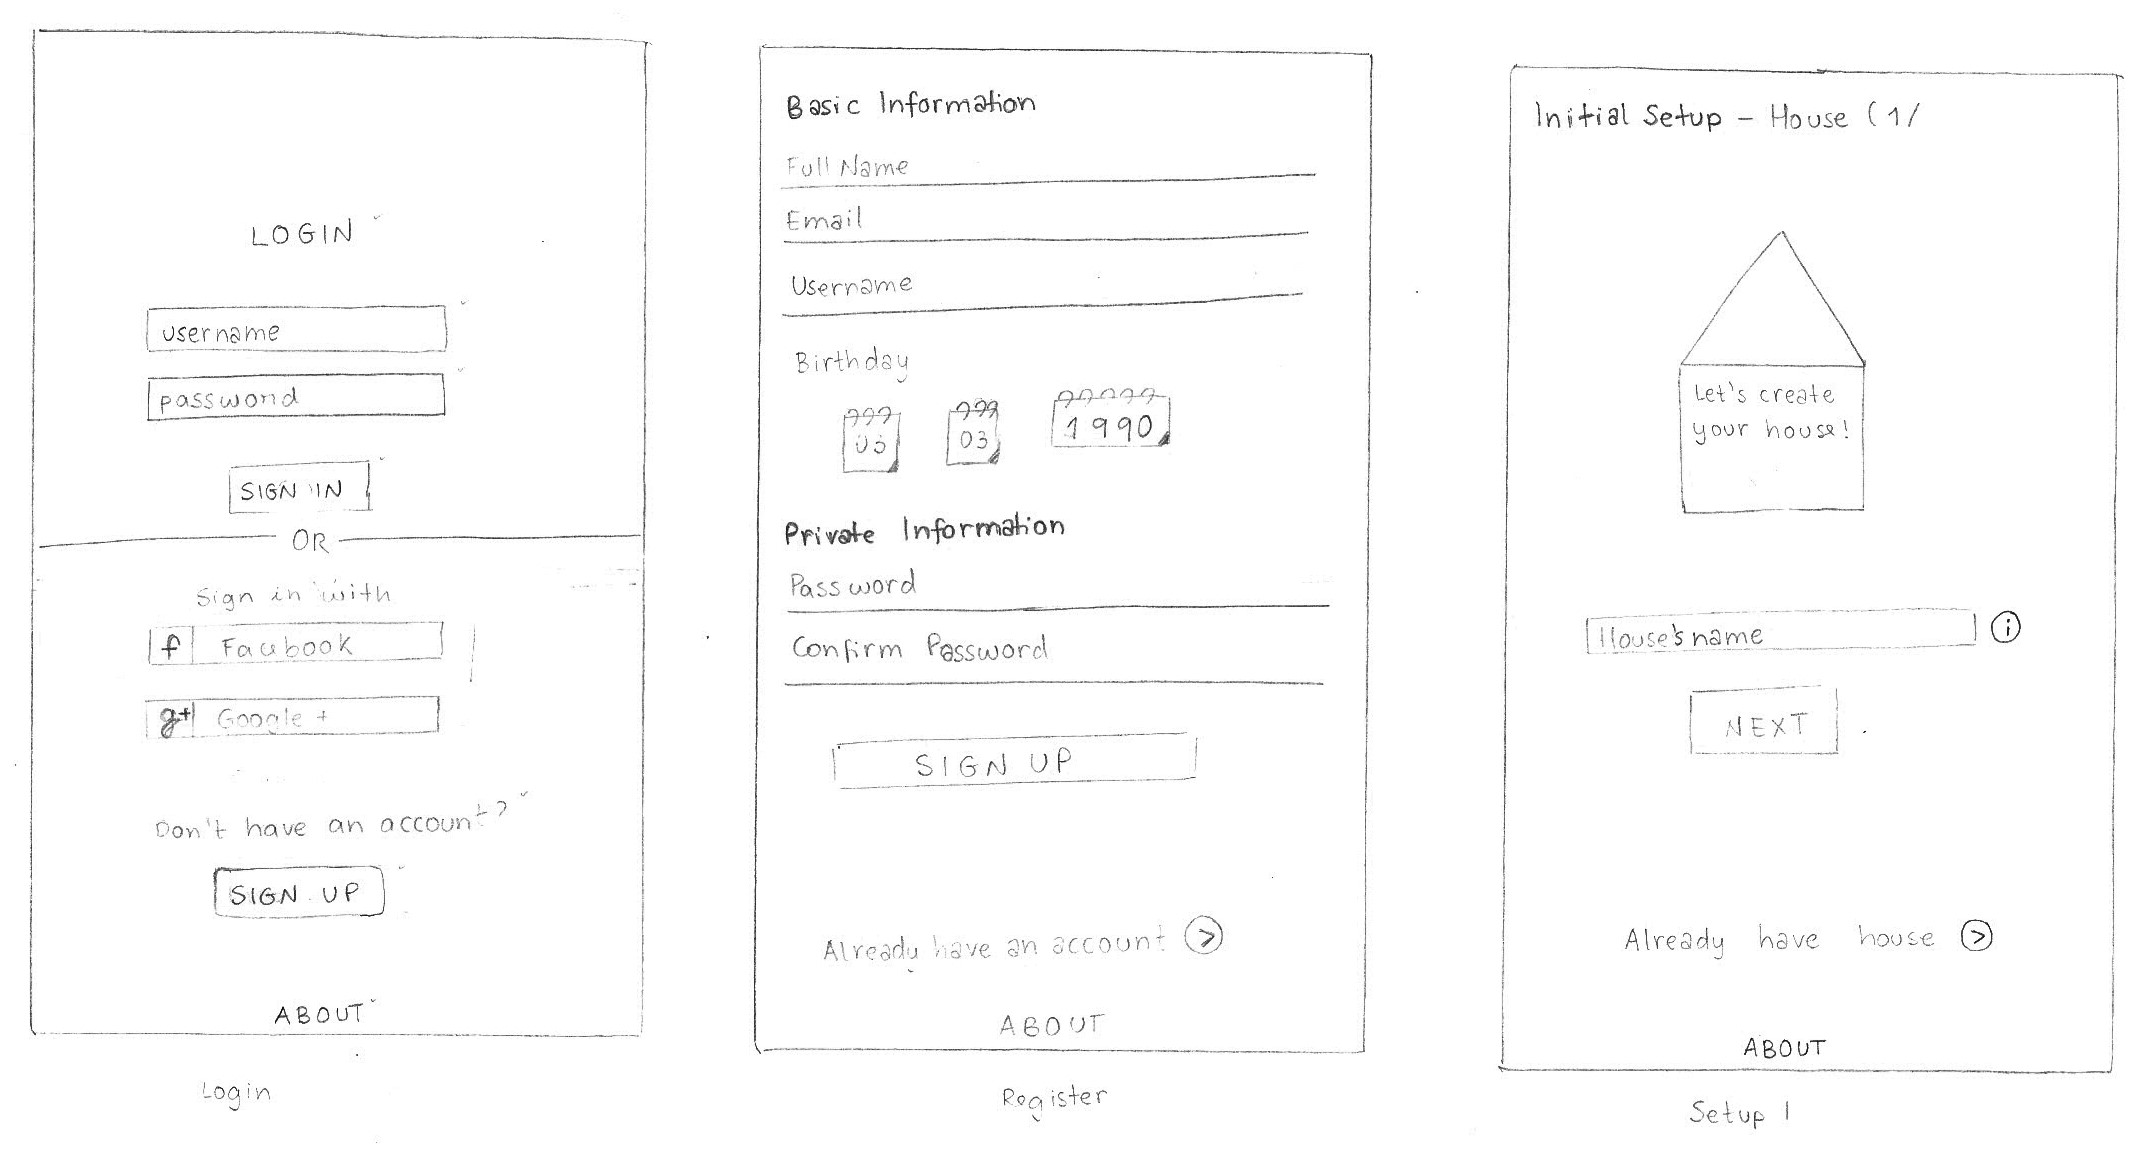
\includegraphics[width=13cm, scale=1]{img/wireframe_1.jpg}
	\caption{Esboço 1}
	\label{wireframe1}
\end{figure}

\begin{figure}[H]
	\centering
	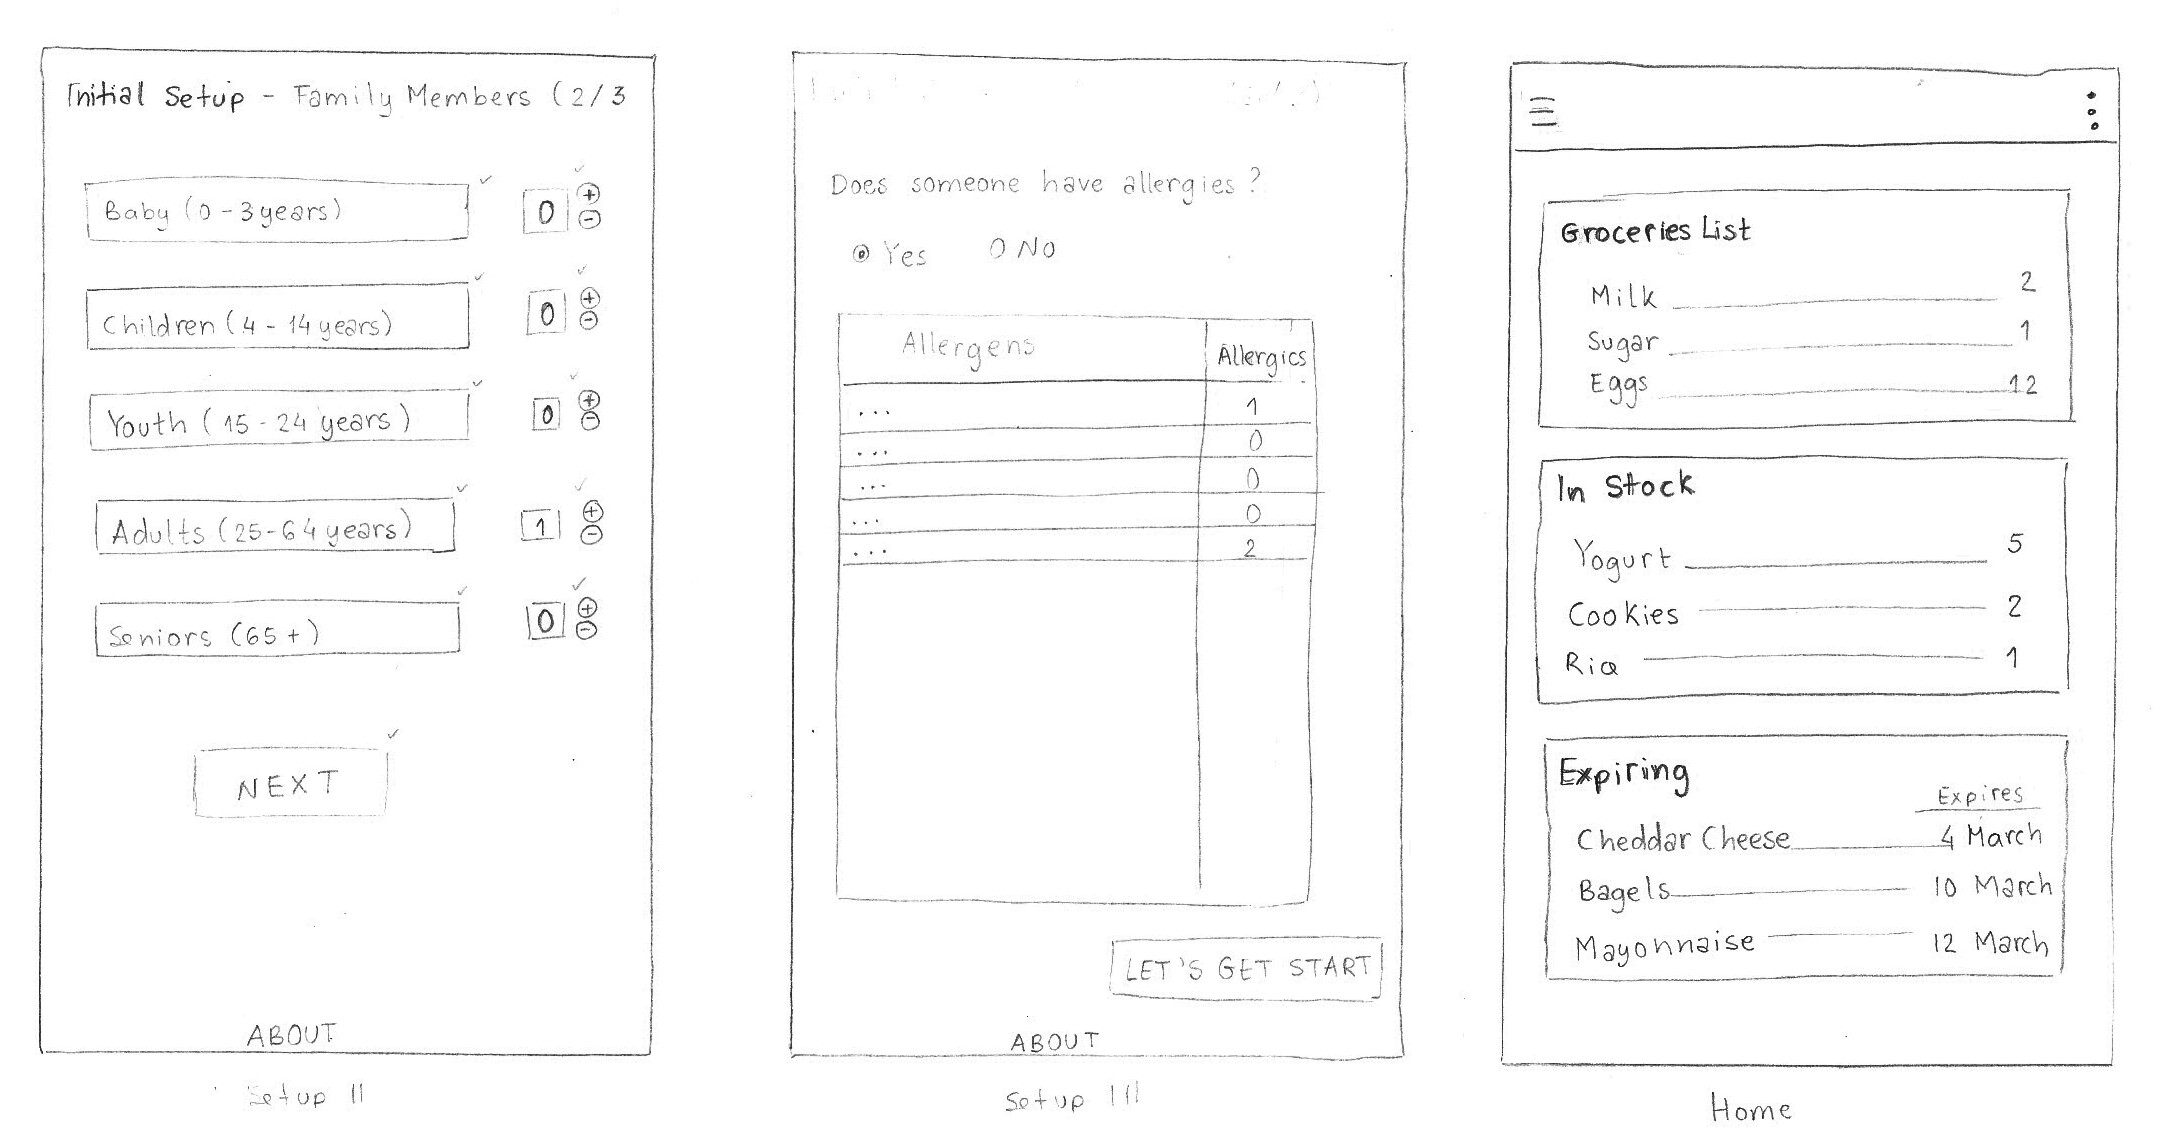
\includegraphics[width=13cm, scale=1]{img/wireframe_2.jpg}
	\caption{Esboço 2}
	\label{wireframe2}
\end{figure}

\begin{figure}[H]
	\centering
	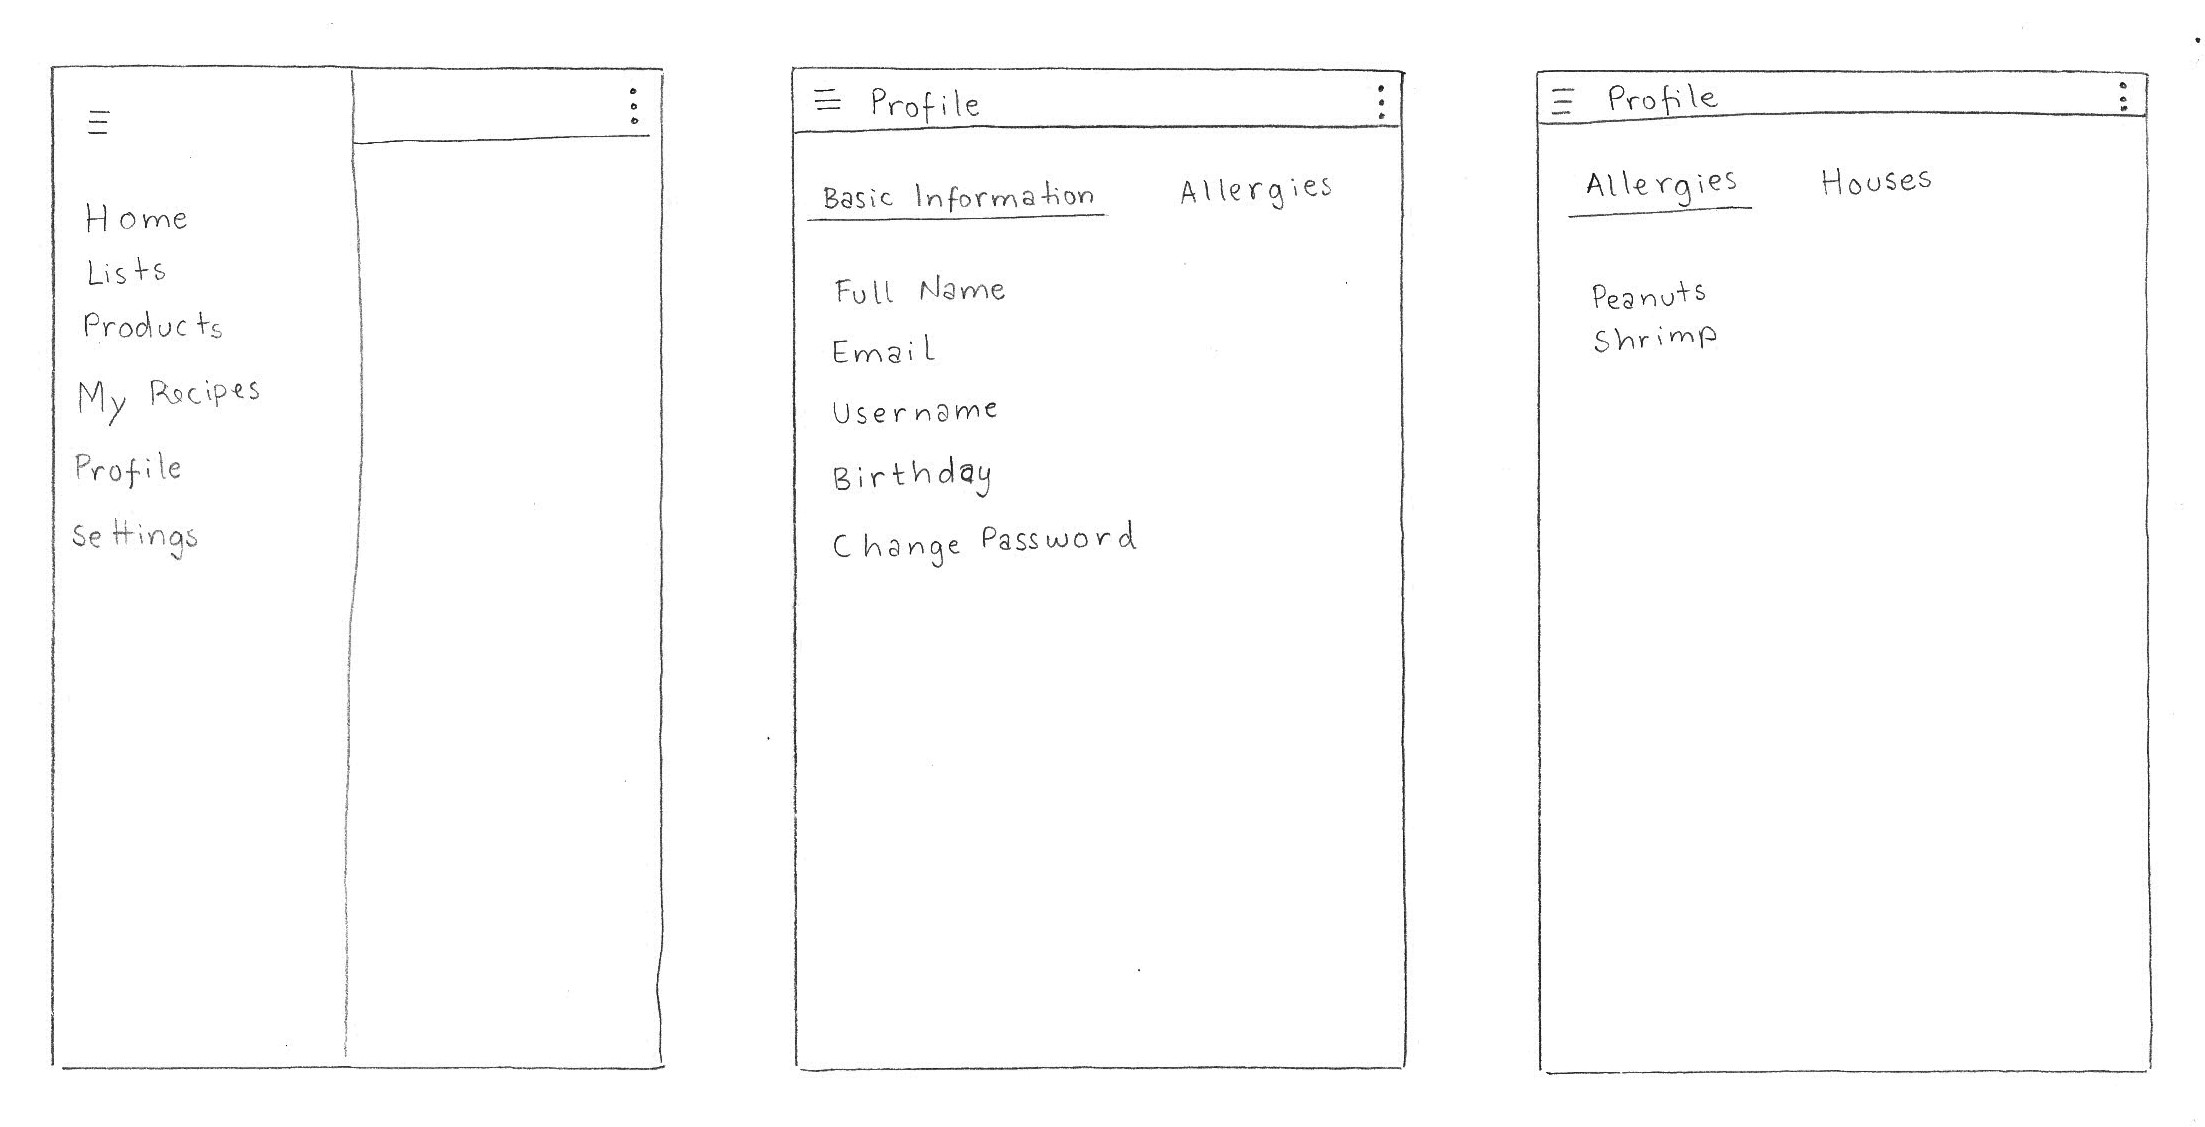
\includegraphics[width=13cm, scale=1]{img/wireframe_3.jpg}
	\caption{Esboço 3}
	\label{wireframe3}
\end{figure}

\begin{figure}[H]
	\centering
	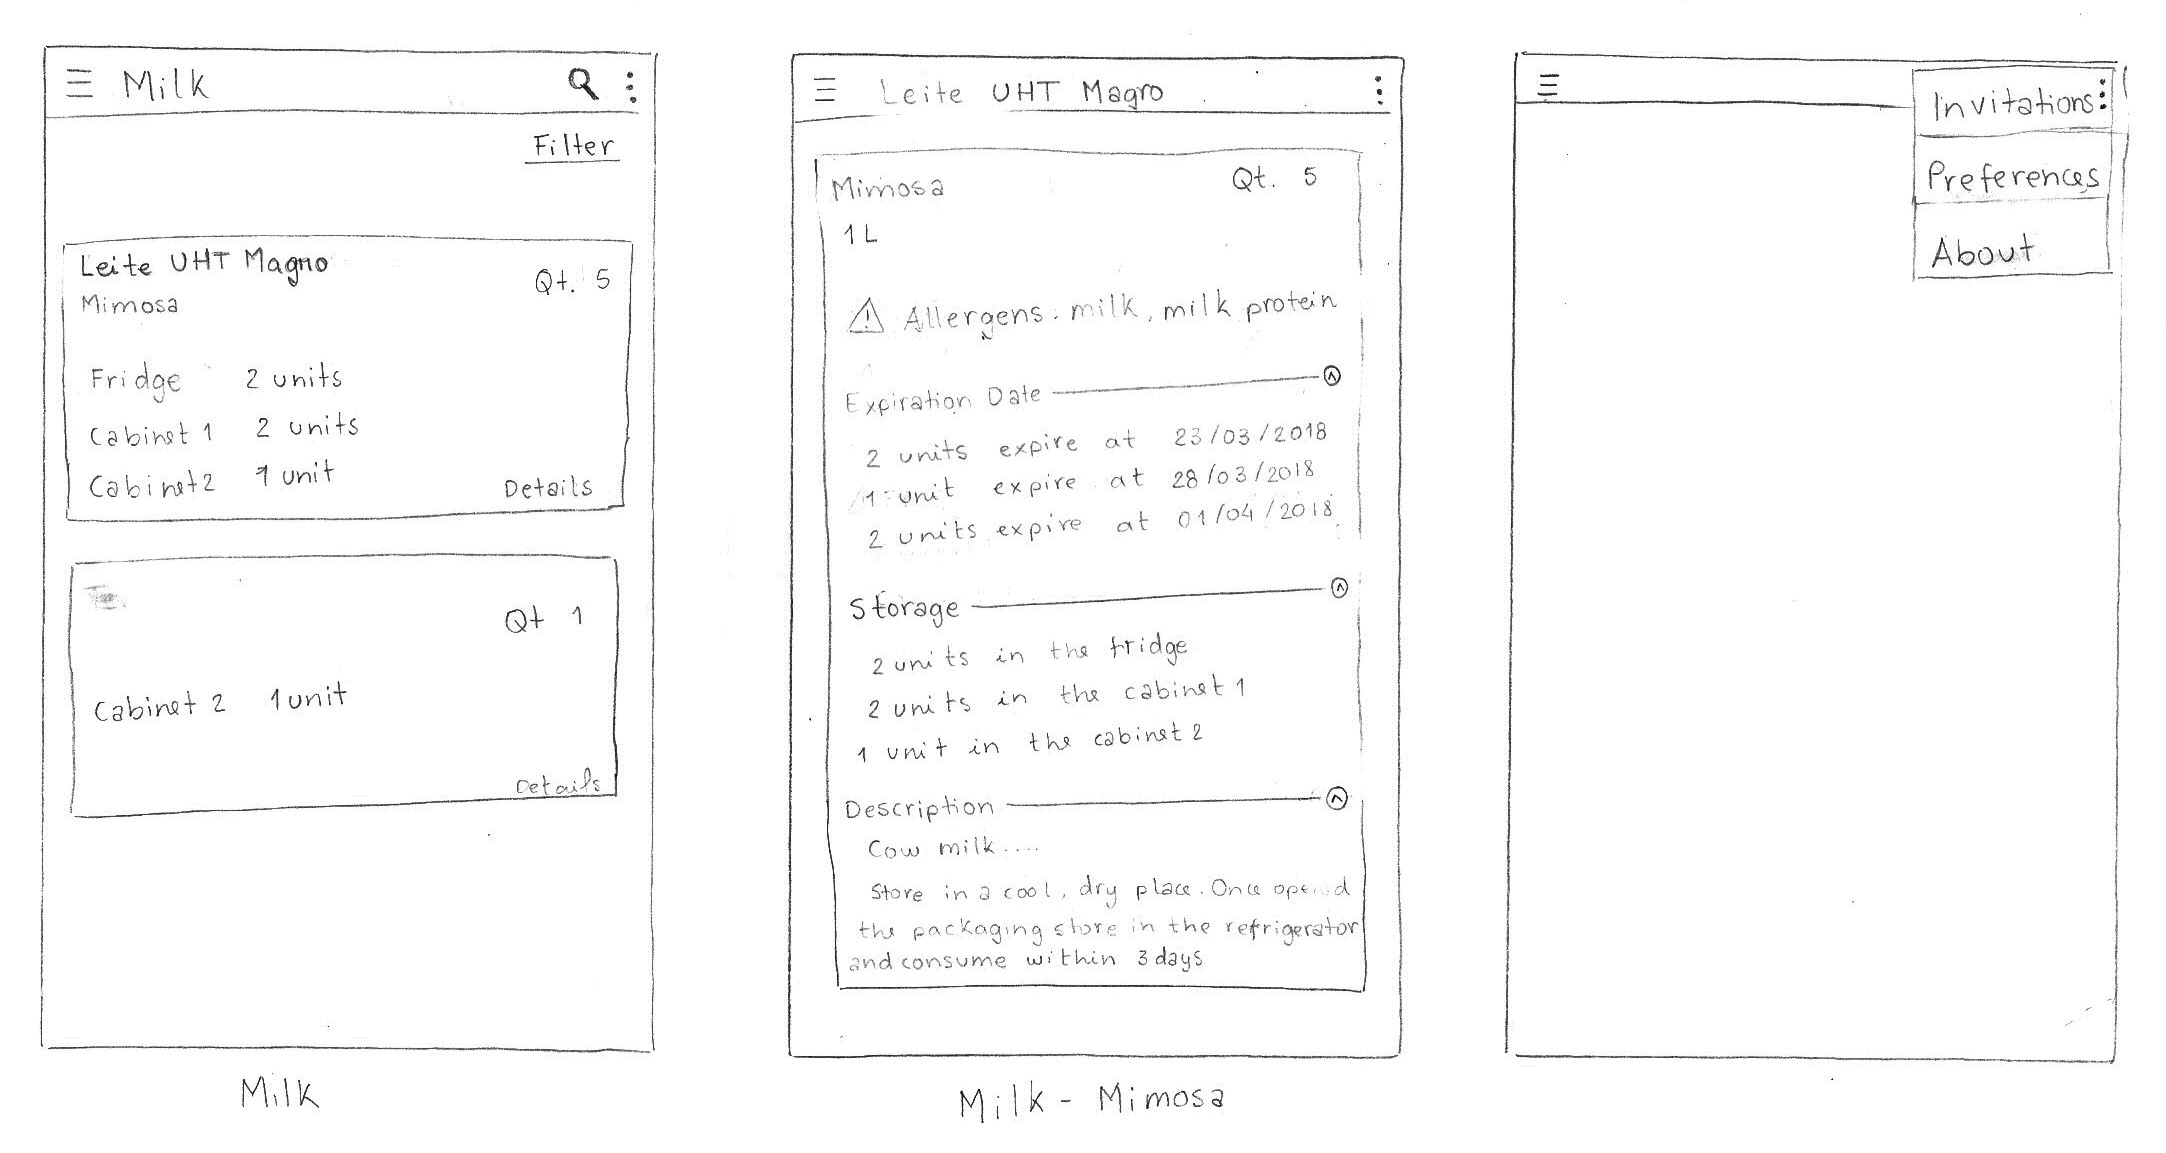
\includegraphics[width=13cm, scale=1]{img/wireframe_4.jpg}
	\caption{Esboço 4}
	\label{wireframe4}
\end{figure}

\begin{figure}[H]
	\centering
	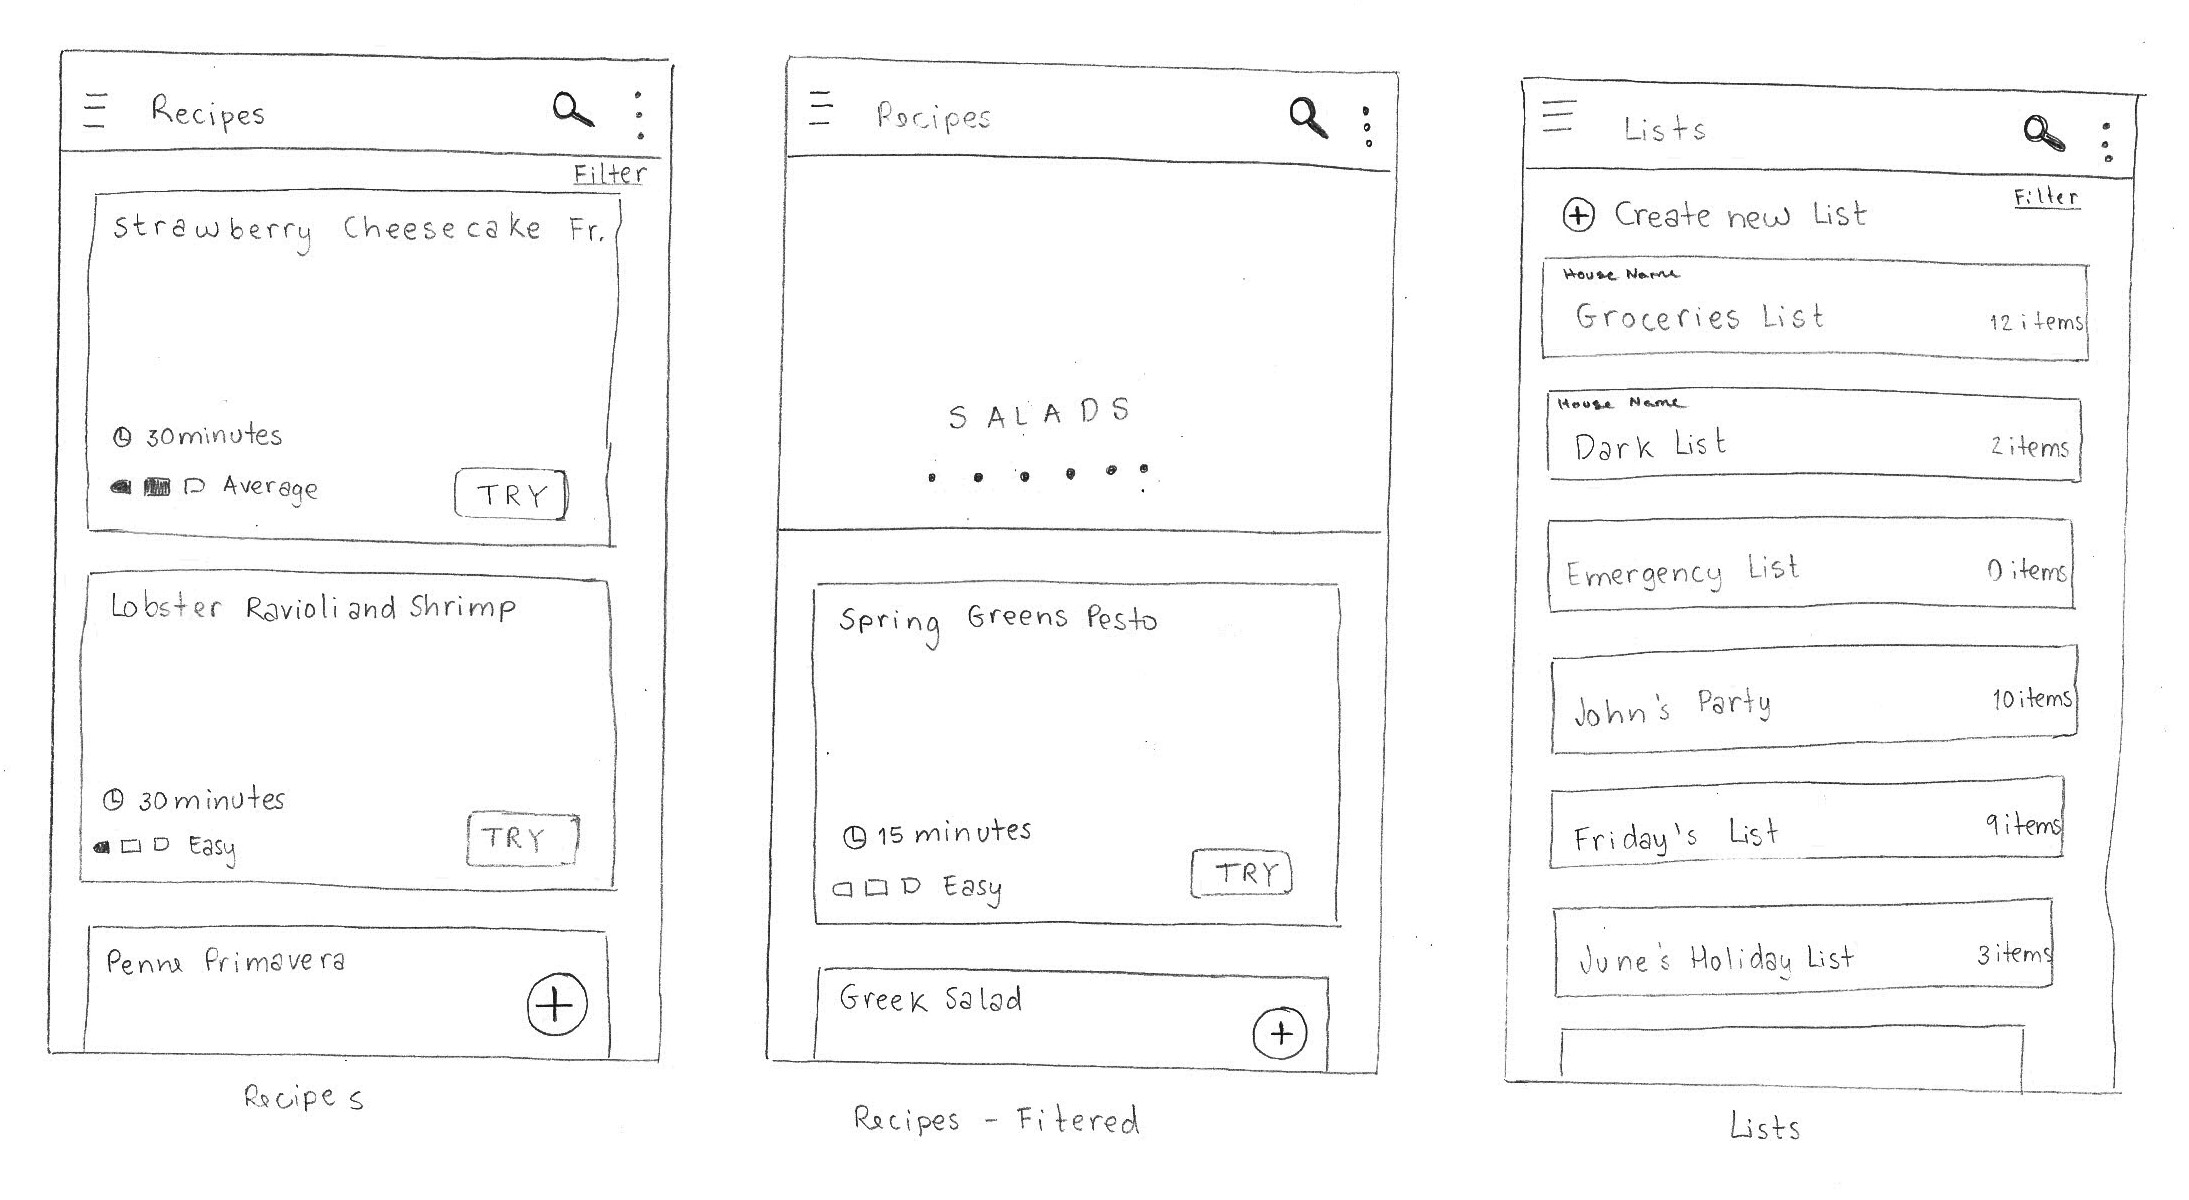
\includegraphics[width=13cm, scale=1]{img/wireframe_5.jpg}
	\caption{Esboço 5}
	\label{wireframe5}
\end{figure}

\begin{figure}[H]
	\centering
	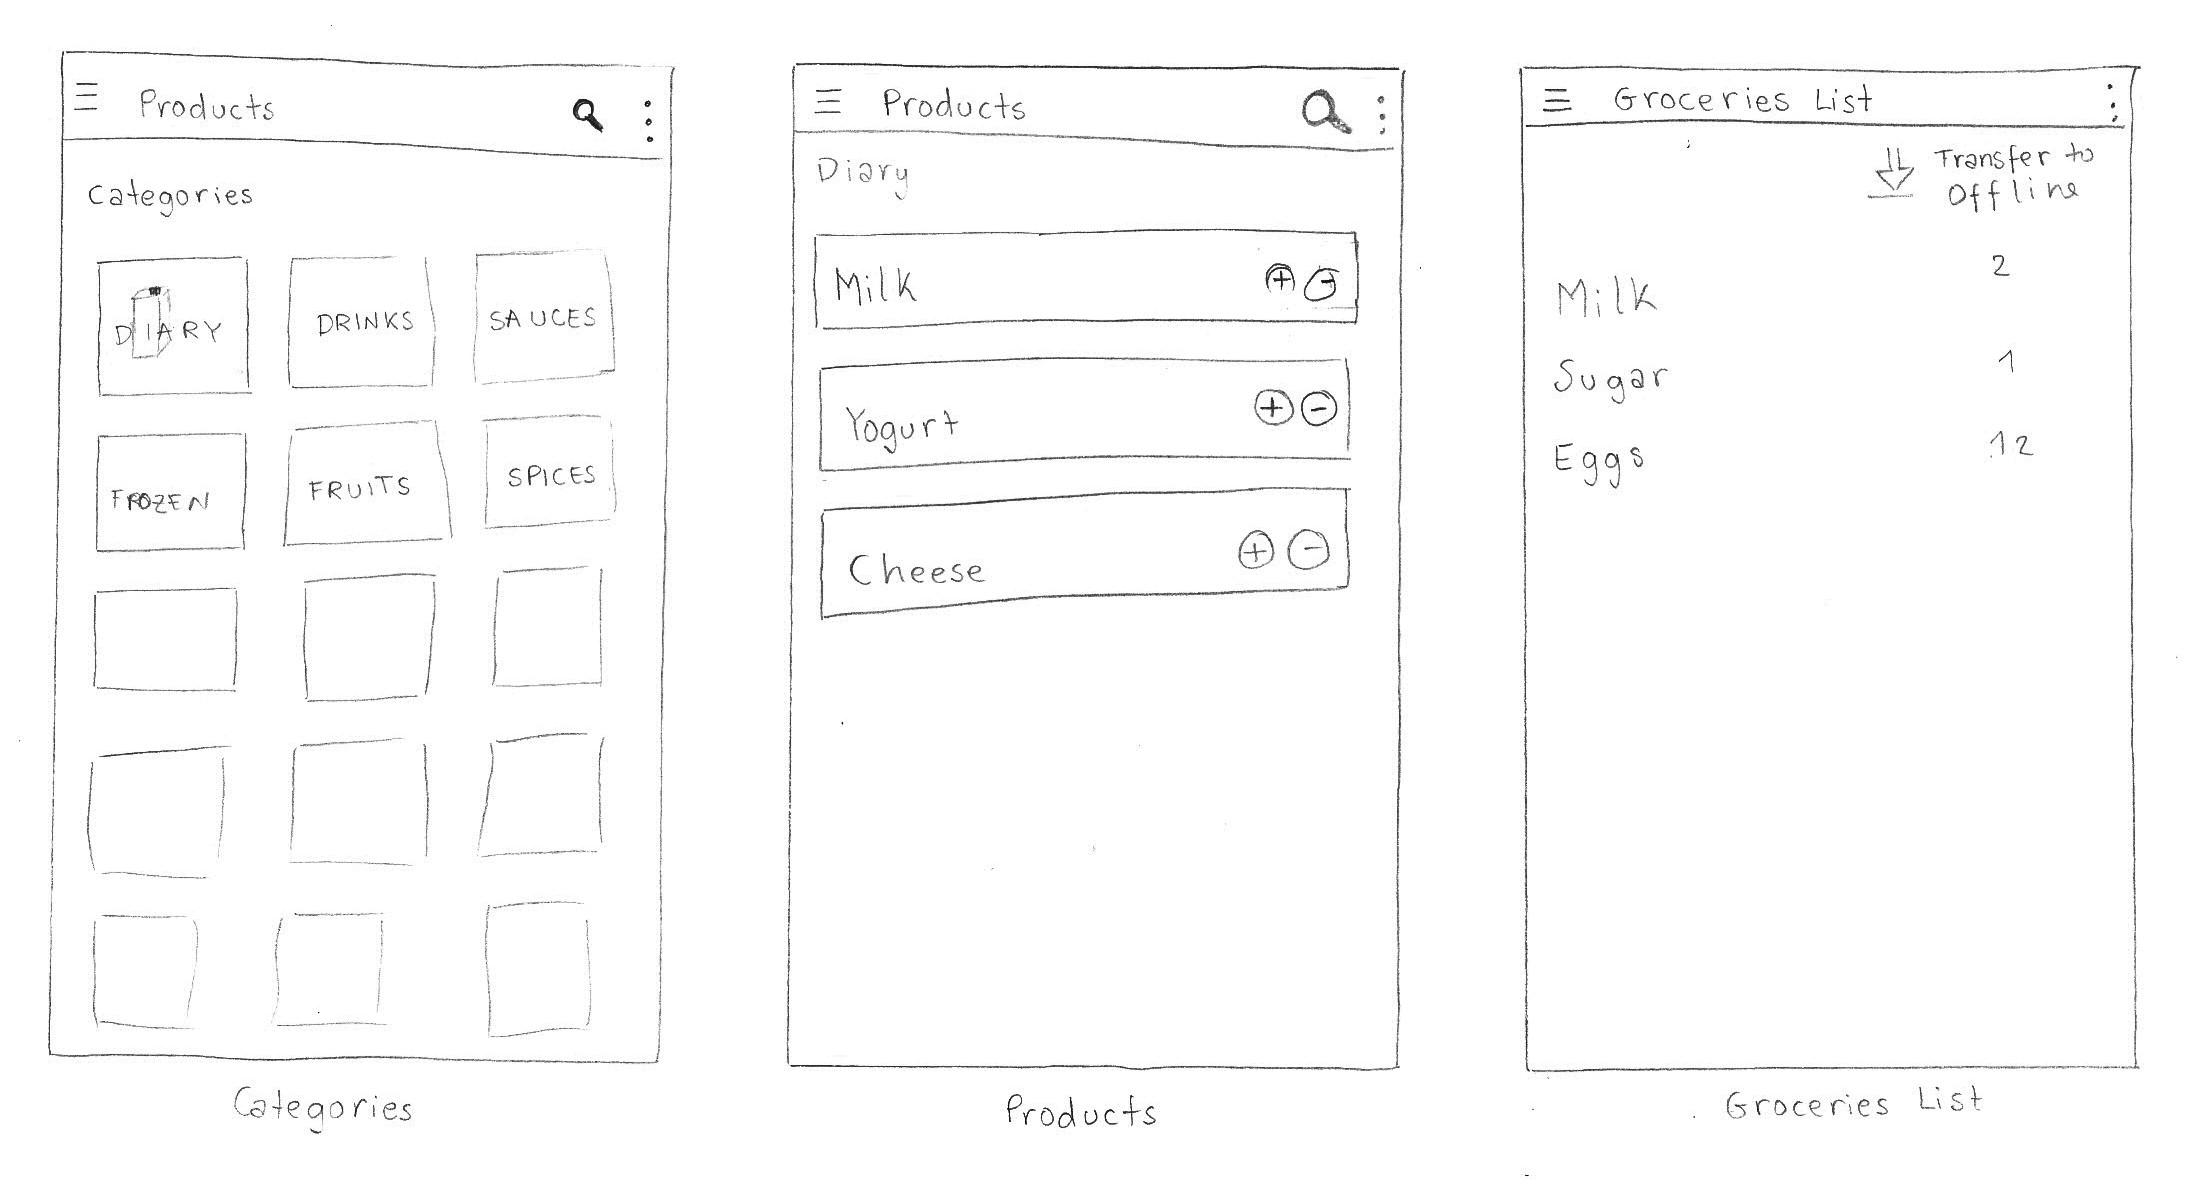
\includegraphics[width=13cm, scale=1]{img/wireframe_6.jpg}
	\caption{Esboço 6}
	\label{wireframe6}
\end{figure}

\begin{figure}[H]
	\centering
	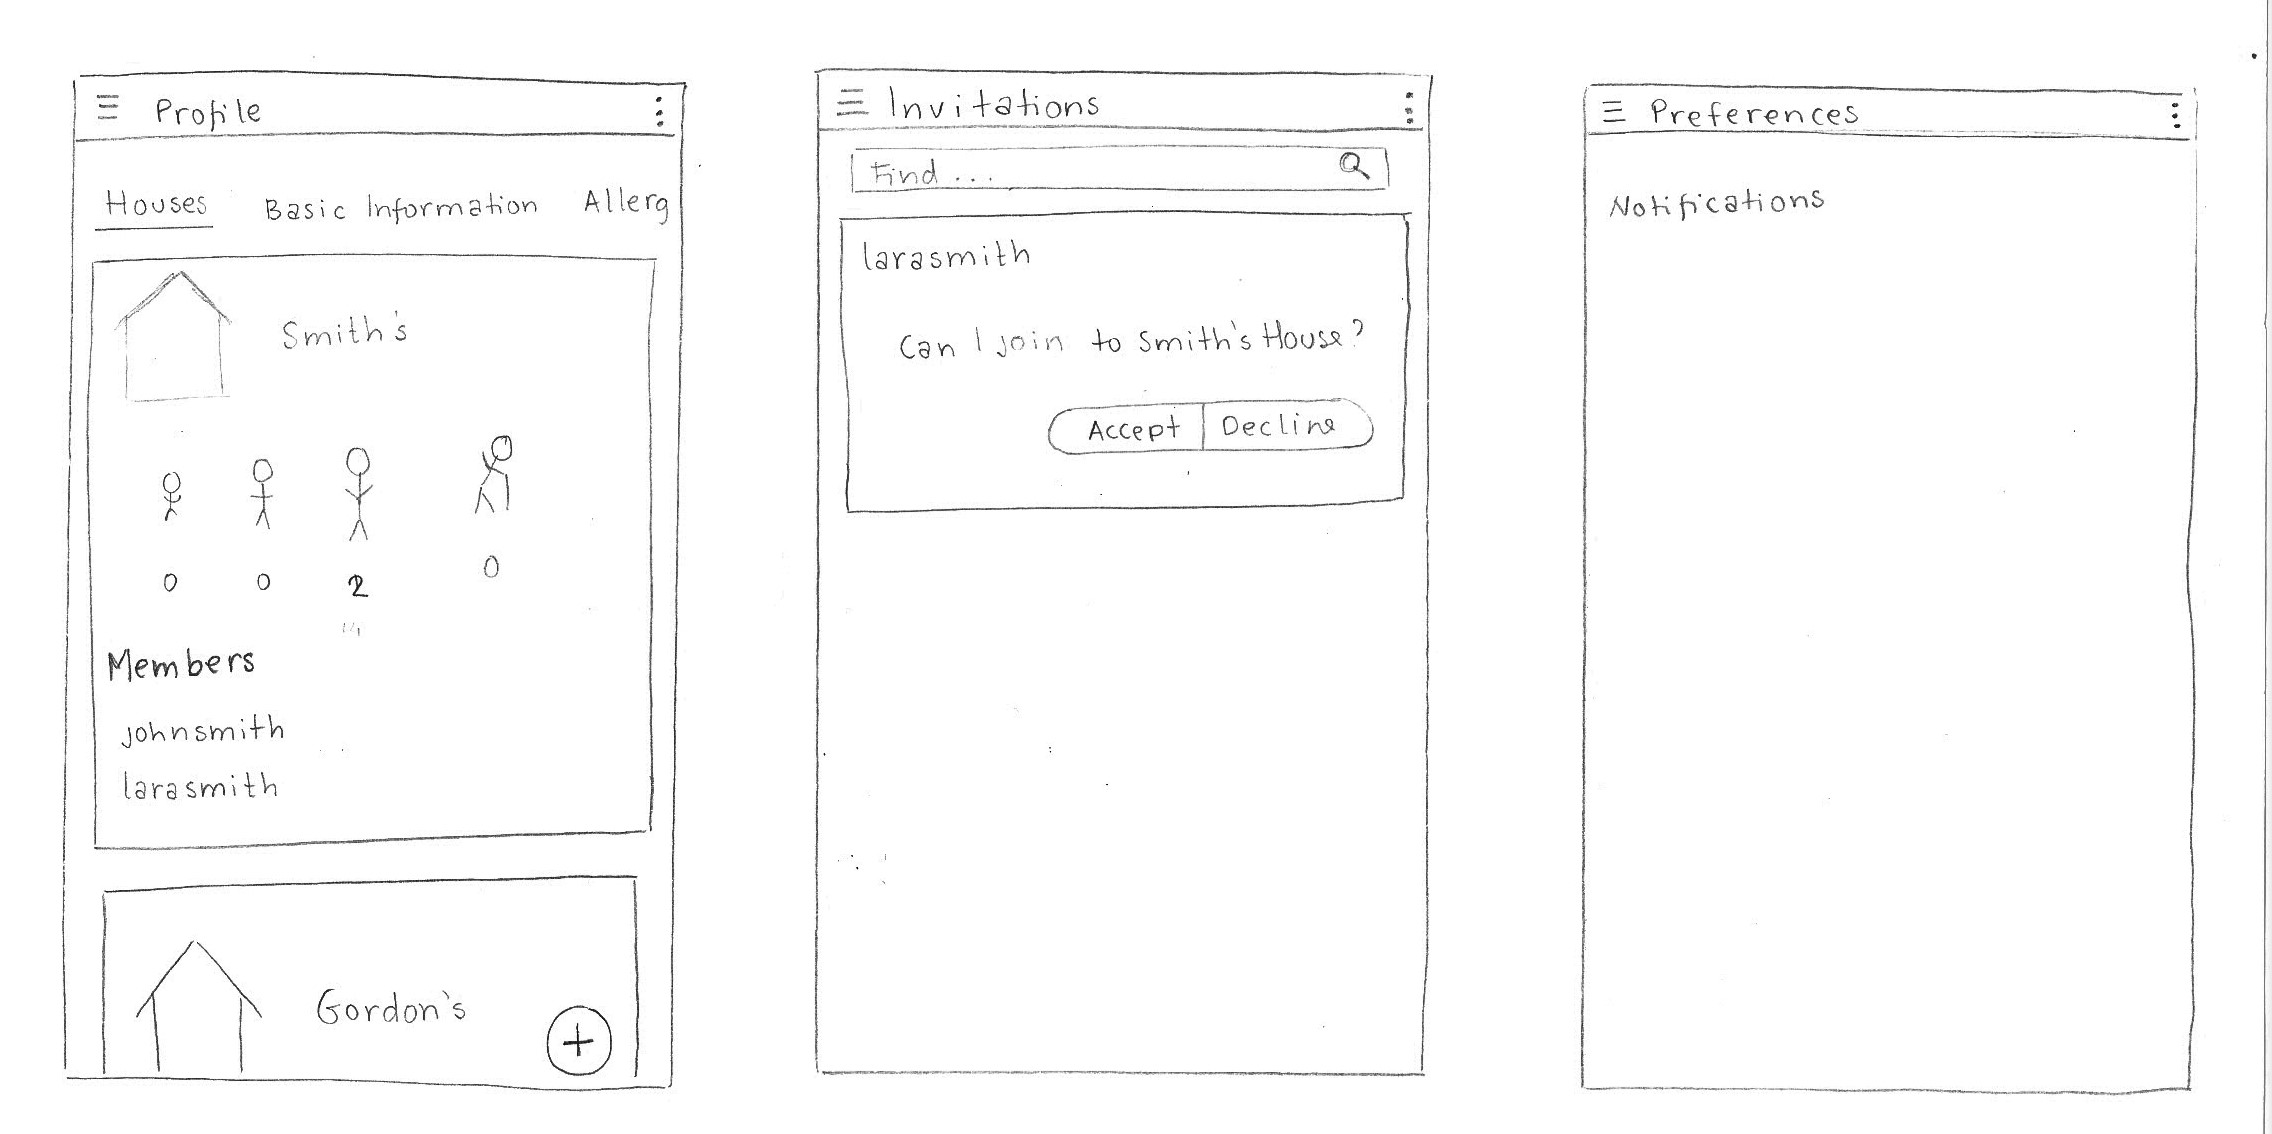
\includegraphics[width=13cm, scale=1]{img/wireframe_7.jpg}
	\caption{Esboço 7}
	\label{wireframe7}
\end{figure}


\subsubsection{Padrões de Desenho}

\textbf{MVC \textit{vs} MVP \textit{vs} MVVM}

Os padrões de desenho em \textit{Android} têm vindo a evoluir, de forma a tornar os componentes independentes e facilmente testáveis. Um dos primeiros padrões a surgir foi o padrão \acrfull{mvc}, porém nos últimos anos, emergiram dois novos padrões, a destacar o \acrfull{mvp} e o \acrfull{mvvm}. Estes padrões elevaram-se com o propósito de evitar a dispersão da lógica de negócio entre as camadas de dados e as gráficas, logo, reduzindo a duplicação de código. Assim como, facilitam a manutenção dos diversos módulos e a realização de testes unitários. Outro fator de relevo é o facto de permitirem trocar rapidamente de repositório de dados, seja este uma base de dados ou APIs.

Na tabela \ref{tab-comparacao-mvc-mvp-mvvm} apresenta-se uma comparação entre os três padrões, pretendendo-se tornar percetível as vantagens e desvantagens de cada um.

\begin{table} [H]
	\centering
	\caption{Comparação dos Padrões MVC, MVP e MVVM}\vspace{2mm}
	\label{tab-comparacao-mvc-mvp-mvvm}
	\begin{threeparttable}
    	\begin{tabular}{m{8cm}|C{2cm}|C{2cm}|C{2cm}}
    		\textbf{} & \textbf{\acrshort{mvc}} & \textbf{\acrshort{mvp}} & \textbf{\acrshort{mvvm}}\\
    		\hline Separação entre o \textit{Model} e a \textit{View} & \cmark & \cmark & \cmark \\
    		\hline Separação entre a \textit{View} e o \textit{Controller} & \xmark & n.a. & n.a. \\
    		\hline Separação entre a \textit{View} e o \textit{Presenter} & n.a. & \cmark & n.a. \\
    		\hline Separação entre a \textit{View} e o \textit{ViewModel} & n.a. & n.a. & \cmark \\
    		\hline Facilidade em testar o \textit{Model} & \cmark & \cmark & \cmark \\
    		\hline Facilidade em testar a \textit{View} & \cmark & \cmark & \cmark \\
    		\hline Facilidade em testar o \textit{Controller} & \xmark & n.a. & n.a. \\
    		\hline Facilidade em testar o \textit{Presenter} & n.a. & \cmark & n.a. \\
    		\hline Facilidade em testar o \textit{ViewModel} & n.a. & n.a. & \cmark\\
    		\hline Facilidade na manutenção do \textit{Controller} & \xmark & n.a. & n.a.\\
    		\hline Facilidade na manutenção do \textit{Presenter} & n.a. & \xmark & n.a.\\
    		\hline Facilidade na manutenção do \textit{ViewModel} & n.a. & n.a. & \xmark\\
    	\end{tabular}
    	\begin{tablenotes}
            \centering
            \item[] n.a. - Não aplicável
        \end{tablenotes}
    \end{threeparttable}
\end{table}

\textbf{Service Locator}

Ao contrário do padrão atualmente muito utilizado, da injeção de dependências, o \textit{Service Locator} \cite{ServiceLocator:android} permite obter instâncias de serviços, através de um único ponto central na aplicação. É ainda possível trocar de implementações em \textit{runtime} consoante o dispositivo onde a aplicação está a ser utilizada.


\subsubsection{Internacionalização}

Na interface com o utilizador são disponibilizados dois idiomas, Português e Inglês. A internacionalização de uma aplicação em \textit{Android} é relativamente simples, uma vez que existem recursos para cada língua suportada \cite{Supportd:android}, sendo tarefa do \textit{Android} determinar qual o recurso de strings a utilizar consoante a língua local associada ao telemóvel.


\subsubsection{Segurança}

A segurança na aplicação móvel \textit{Android} é assegurada de duas formas, recorrendo às \textit{Shared Preferences} e realizando a autenticação através dos pedidos à \gls{api-web}. 
Armazenar \textit{passwords} no \textit{Android} não é uma tarefa simples, uma vez que este não disponibiliza muitos locais onde se possa armazenar informação sensível. As hipóteses consistiram em armazenar nas \textit{Shared Preferences}, numa base de dados \textit{SQLite} ou no \textit{Keystore} do dispositivo. Existem diferentes formas de efetuar o armazenamento das \textit{passwords}, podendo estas serem guardadas em claro, encriptadas com uma chave simétrica, usando o \textit{Android Keystore}, ou encriptadas com uma chave assimétrica \cite{Bestplacetostorepassword:android}.

As \textit{passwords} armazenadas em claro nas \textit{Shared Preferences} ou numa base de dados \textit{SQLite} não é de todo uma boa ideia, pois se um atacante conseguir aceder ao telemóvel obtém acesso ao ficheiro das \textit{Shared Preferences} ou à base de dados, conseguindo, assim, obter a \textit{password} armazenada. Encriptando a \textit{password} com uma chave simétrica, também, não se trata de uma boa ideia pois a chave iria ficar armazenada no \acrfull{apk}. Se um atacante fizer o \textit{decompile} do \acrshort{apk} pode encontrar a chave e assim desencriptar a password. Para além de que a encriptação da \textit{password} consistiria num custo adicional. 

A outra opção passaria por usar o \textit{Android} \textit{Keystore} para encriptar as palavras-chave utilizando uma chave assimétrica. Porém, mais uma vez um atacante com acesso privilegiado (\textit{root}), visto que o \textit{Android} se baseia num sistema \textit{Linux}, conseguiria localizar a chave privada e assim aceder à \textit{password}. Uma opção mais viável seria armazenar a chave privada remotamente e sempre que fosse necessário desencriptar a \textit{password}, esta seria remetida para o servidor que compreende a chave privada para a desencriptação. Esta opção, também, não é a melhor pois necessita de aceder à \textit{password} do utilizador sempre que se realizar um pedido à \gls{api-web}, visto que é necessário enviar no \textit{header} \acrshort{http} \textit{Authorization} as credenciais do utilizador. Outro contra, é no momento do \textit{login} ser necessário fazer um pedido ao servidor fornecedor da chave privada para obter a \textit{password} e realizar o \textit{login} na \gls{api-web}, o que limitaria o futuro da aplicação móvel no sentido de só ser possível o uso desta com Internet. 

Existe ainda outra solução, que seria usar o \textit{Smart Lock for Passwords} da \textit{Google} \cite{SmartLock:android}. Esta foi, igualmente, descartada pela razão anterior de que é necessário ter acesso à Internet para obter a \textit{password}. 

A solução implementada foi armazenar as \textit{passwords} em claro nas \textit{Shared Preferences}, no entanto, este é, sem dúvida, um ponto a melhorar futuramente, por exemplo, passando por utilizar um servidor de autorização do sistema Smart Stocks, em que os utilizadores podem iniciar sessão e em caso de sucesso seria armazenado um \textit{token} na aplicação móvel.

As credenciais são solicitadas ao utilizador no \textit{loggin} e no registo. No caso destes serem sucedidos, a sessão fica iniciada ao longo do tempo, dado que as suas credenciais ficam registadas nas \textit{Shared Preferences}.

O início de sessão é realizado efetuando um pedido à \gls{api-web}, este pedido é autenticado através do \textit{header} \textit{Authorization} e fazendo uso das credenciais inicialmente solicitadas. Em caso do pedido suceder significa que o \textit{loggin} pode ser efetuado com sucesso, caso contrário verifica-se se pode ter sido um erro de credenciais incorretas para assim puder informar o utilizador, ou se se trata de um outro problema.

\subsubsection{Implementação}

A aplicação móvel foi desenvolvida com a linguagem \textit{Kotlin}, pois esta linguagem é: 
\begin{itemize}
    \item concisa,
    \item \textit{null-safe}, por omissão,
    \item interoperável, existindo enumeras bibliotecas da JVM, do \textit{Android} e dos \textit{browsers},
    \item suportada por vários IDEs,
    \item empresas como o \textit{Pinterest}, a \textit{Uber}, a \textit{Evernote}, etc. estão a utilizar linguagem Kotlin em diversas componentes das suas aplicações e programas,
    \item entre muitas outras vantagens \cite{WhyKotlin:kotlin}.
\end{itemize}

\begin{figure}[H]
	\centering
	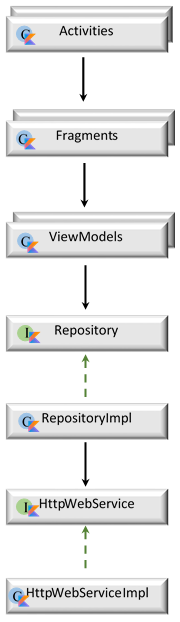
\includegraphics[scale=1]{img/uml.png}
	\caption{Arquitetura da Aplicação Móvel}
	\label{mobile-app-architecture}
\end{figure}

Na Figura \ref{mobile-app-architecture} expõe-se o \acrfull{uml} geral dos componentes da aplicação móvel. Assim de uma forma geral, a arquitetura é composta por \textit{Activities}, sendo a principal a controladora das transações entre fragmentos. Estes últimos utilizam \textit{ViewModels} na obtenção, inserção e remoção de dados, registando-se como observadores da resposta. Os \textit{ViewModels} recorrem ao Repositório para efetuarem as operações básicas \acrshort{crud}. É no repositório que se definem os métodos \acrshort{http} a utilizar e todas as partes integrantes de um pedido \acrshort{http}. Por fim o pedido é efetuado por uma implementação de \textit{HttpWebService}, responsável por adicionar os pedidos a uma fila. Para a realização de pedidos à \gls{api-web} utilizou-se a biblioteca \textit{Volley} \cite{Volley:android}, esta biblioteca permite realizar pedidos de forma rápida, simples e assíncrona a \textit{REST-Clients}.

%https://medium.com/@magnus.chatt/why-you-should-totally-switch-to-kotlin-c7bbde9e10d5

%https://www.quora.com/What-are-the-advantages-of-Kotlin-over-Java


\subsection{Aplicação \textit{Web}}

A aplicação \textit{web} foi pensada como uma aplicação de consulta, onde facilmente os utilizadores podem aceder, através dos diversos \textit{browsers} existentes, aos dados relativos às suas casas. Primeiramente pensou-se em desenvolver a aplicação recorrendo ao ambiente \textit{Node.js} com o auxílio da \textit{framework} \textit{Express}, contudo esta deve ser utilizada para desenvolver \gls{api-web} o que não era o pretendido. Deste modo, optou-se pelo o uso da biblioteca \textit{React}, que é amplamente empregue na criação de \textit{user interfaces} \cite{ReactvsExpress:web}.


\subsubsection{Internacionalização}

A aplicação \textit{Web} apenas está disponível no idioma Português.


\subsubsection{Segurança}

À semelhança da aplicação móvel a autenticação é efetuada nos pedidos através do \textit{header Authorization}. A sessão apenas permanece enquanto a janela estiver aberta, para este efeito utiliza-se a propriedade do \textit{Session Storage}.
